\section{Raspberry PI}
Attention Tracker is a module which can be installed independently on show cases, merchandise, posters to see which product is getting maximum attention from people. It is completely unobtrusive unlike survey forms and feebdack requests and therefore can be more effective. It uses Face recognition software called opencv, an image processing algorithm, and neural network. This application is on top of
raspbian os which controls the frequency of monitoring, raspbian os is an open source oeprating system for Raspberry PI, based on linux kernel. It is a branch of debian OS. The module, works by capturing images of objects, temporarily storing them on disk and processing them to see if image of a face exists in the stored image. After detection stored images is immediately deleted or over written to conserve space. 

\begin{figure}[!ht]
\centering
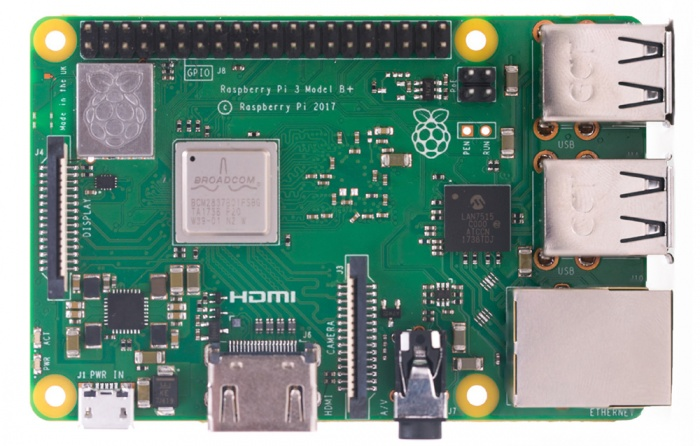
\includegraphics[scale=0.7]{raspberrypi}
\caption{Raspberry pi 3 b+}
\end{figure}


From opencv we use feature extraction a feature extraction method, which subtracts pixels of a group(identified by the algorithm) from
the original image, to form a pattern object. This pattern object is then subjected to neural network to check if it fits the pattern of a face. It is based on the work done by Witsarut Sriratana et al\cite{opencv}.
